\documentclass[times, utf8, zavrsni]{fer}
\usepackage{booktabs}
\usepackage{listings}
\usepackage{tgcursor}
\lstset{basicstyle=\sffamily\selectfont}
\graphicspath{ {images/} }

\begin{document}

\thesisnumber{000}

\title{Sustav za izdvajanje tabličnih podataka iz web-stranica}

\author{Stanko Krtalić Rusendić}

\maketitle

\zahvala{Hvala Veljku i Klemi na ukazanom povjerenju}

\tableofcontents

\chapter{Uvod}



\chapter{Postojeća rješenja}

\section{Uvod}

Postoji nekolicina, javno dostupnih, gotovih rješenja za izdvajanje tabličnih
podataka iz PDF \cite{pdf_documentation}
i HTML \cite{html_documentation}
datoteka. Svako od rješenja ima prednosti i mane koje je
bitno proučiti prije razrade i implementacije vlastitog rješenja.

\section{Tabula}

Tabula \cite{tabula_repository} je rješenje otvorenog koda napisano u
programskom jeziku JRuby \cite{jruby_documentation}.
Nudi grafičko sučelje tako sto pokrene poslužitelj preko kojeg poslužuje web
aplikaciju i sučelje za naredbeni redak kroz
JAR \cite{java_language_specification} datoteku. Moguće je vaditi
tablične podatke jedino iz PDF dokumenata koji su tekstualnog tipa, odnosno,
ne posjeduje mogućnosti prepoznavanja teksta i tablica iz slika.

JRuby je verzija programskog jezika Ruby namijenjena izvođenju na Java
virtualnom stroju \cite{java_virtual_machine_specification} (eng. kratica JVM).
To JRubyju omogućuje korištenje
programskih knjižnice iz ostalih jezika koji se izvršavaju na JVM-u. Tako
Tabula za parsiranje PDF dokumenata koristi knjižnice JPedal i Apache
PDFToolbox \cite{apache_pdftoolbox_specification} napisane u programskom
jeziku Java \cite{java_language_specification}.

Interno, aplikacija pretražuje PDF dokument za tabličnim objektima koje potom
pretvara u CSV zapis i pohranjuje kao datoteku.

Najveće manjkavosti ovog rješenja su ne-interaktivno sučelje naredbenog redaka,
činjenica da se izvodi kao zaseban proces (poslužitelj) sto zahtijeva od
korisnika
da koristi internet preglednik i ovisnost o lokalnoj instalaciji JVM-a.

\section{pdftabextract}

pdftabextract \cite{pdftabextract_repository} je rješenje otvorenog koda napisano
u programskom jeziku Python.
Nudi isključivo sučelje naredbenog redaka i ne može direktno obrađivati PDF
datoteke, već ih je prethodno potrebno konvertirati u pdf2xml format.

Korištenje programskog alata pdf2xml omogućava ovom rješenju reparaciju
podataka prije nego li ih krenemo obrađivati. Moguće reparacije su rotacija
stranice, ispravka iskrivljene slike i razdvajanje dvostrukih stranica. Ovaj
korak je iznimno bitan kako rješenje ne konzumira strukturirane podatke već
pokušava otkriti grupe podataka koje su vizualno organizirane u redove i
stupce, te ih organizirati u CSV datoteku.

Takav pristup obradi PDF datoteka omogućava pdftabextractu rad s dokumentima
koji su bili konvertirani iz slike u text, te dokumente koji nemaju strogo
definiran tablični format.

Međutim nedostatak ovakvog pristupa je nepouzdanost.
CSV datoteke, koje ovo rješenje vraća kao rezultat, često izgledaju ne
strukturirano i potrebno je ručno sanitizirati rezultat. Također, iz testiranja
sam ustanovio da često krivo zaključi koji podaci pripadaju retku tablice.
Tako će, na primjer, podatak koji zauzima vise redaka unutar jedne ćelije
tablice biti pretvoren u vise ćelija, tj. redaka u tablici.

\section{PDFFigures 2.0}

PDFFigures 2.0 \cite{pdffigures_2_repository} je rješenje otvorenog koda
napisano u programskom jeziku Scala \cite{scala_documentation}. Slično kao
pdftabextract nudi isključivo
sučelje naredbenog redaka, ali može direktno procesirati PDF datoteke. Fokus
rješenja je na ekstrahiranju podataka iz znanstvenih radova u polju računalne
znanosti.

Rezultat koji ovo rješenje vraća je skup podataka koji opisuju figure PDF
dokumenta. Sve sto nije isključivo kvadrat s tekstom se interpretira kao
figura, npr. slike, tablice, ilustracije i slično.

Manjkavosti ovog rješenja slične su onima od Tabule \cite{tabula_repository}.
Za pokretanje je potrebno
imati instaliraju točnu verziju JVM-a, ne postojanje interaktivnog sučelja i
potreba za dodatnim eksternim programskim knjižnicama. Također, sučelje
naredbenog redaka je nezgrapno za korištenje kako se svodi na pisanje Scala koda
koji se predaje Java virtualnom stroju na izvođenje.

\section{PDFLayoutTextStripper}

PDFLayoutTextStripper \cite{pdflayouttextstripper_repository} je programska
knjižnica otvorenog koda napisano u programskom jeziku Java.

Za razliku od prethodno navedenih rješenja primarna svrha ovog rješenja nije
ekstrahiranje tabličnih podataka, već ekstrahiranje teksta i očuvanje njegovog
prostornog rasporeda.

Ima sposobnost direktne obrade PDF datoteka (sto uspijeva pomoću knjižnice iz
Apache PDFToolboxa).

Ova knjižnica ima iste nedostatke kao i Tabula \cite{tabula_repository} i
PDFFigures 2.0 \cite{pdffigures_2_repository}, te dodatno ne
nudi nikakvo sučelje za direktno korištenje već je potrebno implementirati
vlastito programsko sučelje.



\chapter{Idejno rješenje}

\section{Uvod}

Iz pregleda postojećih rješenja moguće je izdvojiti tri zajedničke mane.

\begin{itemize}
  \item Sva rješenja zahtijevaju da korisnik ima instaliran neki virtualni
    stroj i dodatne  programske knjižnice
  \item Nedostatak kvalitetnog i univerzalnog sučelja (bilo grafičkog ili iz
    naredbenog redaka)
  \item Ne praćenje UNIX filozofije \cite{unix_philosophy}
\end{itemize}

pdftabextract donekle prati UNIX filozofiju i koristiti drugu aplikaciju kako bi
pretvorio PDF datoteke u pdf2xml format koji se lako parsira i obrađuje.

HTML datoteke je lakše parsirati i obrađivati od PDF datoteka kako je njihov
sadržaj strukturiran i jasno definiran.
Stoga bi konačno rješenje, u svrhu
jednostavnosti izvedbe i poboljšanja rezultata, trebalo isključivo
implementirati podršku za obradu HTML datoteka.

Za obradu PDF datoteka, ili bilo kojeg drugog tipa datoteke,
potrebno je istu prethodno pretvoriti u HTML datoteku pomoću alata poput
pdf2htmlEX \cite{pdf2htmlex_repository}.

\section{Željena funkcionalnost}

\subsection{Podržani tipovi ulaznih podataka}

Prethodno su navedene prednosti korištenja podataka zapisanih u HTML formatu.
Konačno rješenje ne bi smjelo biti ograničeno isključivo na HTML podatke već
bi trebalo nuditi mogućnost za lakom nadogradnjom novih formata za slučaj
pojavljivanja formata koji se ne može pretvoriti u HTML ili za slučaj da se
uvidi da je efikasnije direktno podržavati neki format.

Rješenje mora moći primiti podatke direktno preko standardnog ulaza, pročitati
ih iz datoteke ili ih preuzeti s poveznice. Čitanje podataka iz datoteke i
preuzimanje s poveznice ne prati UNIX filozofiju, ali povećava ergonomičnost
rješenja. UNIX filozofija naglašava da bi za obradu podatak iz datoteka i s
poveznica trebali koristiti standardne alate poput cata, seda, curla i wgeta
kako bi predali sadržaj datoteke ili poveznice našem rješenju na standardni
ulaz. Međutim iz iskustva se pokazalo da takvo ulančavanje može stvoriti
kompleksne lance naredbi za postizanje radnje koja je u bilo kojem programskom
jeziku izrazito jednostavno za postignut. Stoga, u svrhu ergonomije i boljeg
korisničkog iskustva, će konačno rješenje podržavati i ne standardne ulaze
podataka.

\subsection{Sučelje naredbenog redaka}

Kroz sučelje naredbenog redaka korisnik može izdvojiti pojedinačnu tablicu i nad
njom izvršiti agregacijske funkcije, ili može izdvojiti sve tablice iz nekog
dokumenta. Time sto je izvoženje agregacijskih funkcija ograničeno na
pojedinačne tablice se smanjuje kompleksnost konačnog rješenja i olakšava se
rad korisniku kako ne mora učiti meta-jezik s kojim bi definirao izvođenje
željenih agregacijskih funkcija nad tablicama - problem uviđen u već postojećim
rješenjima, ali i u drugim alatima poput awk-a.

Osim navedenog mora se nuditi sučelje za izlistavanje tablica u dokumentu
kako bi korisnik mogao odrediti koje tablice želi izdvojiti. Sučelje bi
trebalo prikazati nekolicinu stupaca tablice (koliko korisniku stane na ekran)
i prva 3 retka.  Prethodno je spomenuto da mora postojati i sučelje za
selekciju tablica koje se treba izdvojiti.

\subsection{Grafičko sučelje}

Kroz grafičko sučelje korisnik mora imati sposobnost napraviti sve sto je
moguće i u sučelju naredbenog redaka. Grafičko sučelje bi trebalo predstavljati
interaktivni način rada za sučelje naredbenog redaka. Ovakav pristup će konačno
rješenje učiniti nepristupačnim korisnicima koji ne znaju koristiti sučelje
naredbenog redaka, međutim korisnicima koji znaju koristiti to sučelje će
olakšati proces učenja korištenja alata.

Postoji mogućnost da se stvori puno grafičko sučelje nad opisanim rješenjem.
Implementacija punog grafičkog sučelja bi trebala, preko sistemskog sučelja,
slati naredbe rješenju i koristiti povrate informacije za prikaz vizualnih
elemenata na ekranu. Alternativno, moguće je i razdvojiti jezgru ovog rješenja
od koda zaduženog za interakciju s korisnikom i tako rješenje pretvoriti u
programsku knjižnicu. To bi omogućilo da se isti kod koristi da pogoni razna
sučelja prema korisniku.

\subsection{Podržani tipovi izlaznih podataka}

Rješenje mora nuditi mogućnost zapisa izlaznih podataka u raznim formatima
koji su standardni za tablične podatke - poput csv \cite{csv_documentation},
xls \cite{xls_documentation}, xlsx \cite{xlsx_documentation} i
ods \cite{ods_documentation} formata.
Slično argumentu s ulaznim datotekama, rješenje za izlazne datoteke mora nuditi
pohranu u datoteku i ispis na standardni izlaz. Ponovno, ovakva odluka ne
prati UNIX filozofiju, ali povećava ergonomičnost rješenja.

\section{Arhitektura aplikacije}

Kako bi konačno rješenje bilo nezavisno o nekom virtualnom stroju ili o
programskim knjižnicama potrebno ga je implementirati u programskom jeziku
koji se može prevesti u procesorski kod.

Programske knjižnice se moraju statično povezati u rezultantnu binarnu
datoteku aplikacije kako korisnik ne bi morao prilagođavati svoju programsku
okolinu i instalirati dodatne programske knjižnice da pokrene aplikaciju.

Dinamično povezivanje programskih knjižnica može kod korisnika uzrokovati
nepredviđene probleme poput ne kompatibilnosti dvaju ili više knjižnica i
konflikt u verziji knjižnice između dvaju ili vise aplikacija. Osim toga,
krajnjeg korisnika se tereti s održavanjem instalacije programske knjižnice.

Rješenje se treba moći lako nadograđivati i proširivati. Prethodno je navedeno
postojanje mogućnosti da će rješenje mora podržavati ulazne datoteke
drugačijeg tipa od predviđenih HTML datoteka. Isto razmišljanje može se
primijeniti na izlazne datoteke, te na agregacijske funkcije. Kroz vrijeme će
se pokazati potreba za dodatnim agregacijskim funkcijama ili tipovima izlaznih
datoteka.

S toga konačno rješenje mora implementirati arhitekturu koja
podržava programske dodatke \cite{plugin_architecture_wiki}
(eng. plugin). Ovakvu arhitekturu moguće je
postignuti implementacijom stoga filtera \cite{middleware_wiki}
(eng. middleware stack) ili
implementacijom usmjerivača zahtjeva \cite{router_arhitecture_ieee}
(eng. router).

Kod stoga filtera ulazni podaci se propuštaju kroz skup filtera, svaki filter
obraduje podatke i potom ih predaje sljedećem filteru na obradu. Dok se kod
routera podaci predaju routeru koji ih onda predaje isključivo jednom modulu na
obradu.

Stog filtera je fleksibilnije rješenje, za dodavanje novog filtera potrebno
je implementirati filter i dodati ga na željeno mjesto u stog. Više različitih
filtera može obrađivati isti podatak tako da nema potreba za stvaranjem
monolitnih modula ili duplikacijom logike. Routeri, kao sto je prethodno
navedeno, su manje fleksibilno rješenje. Za dodavanje novog modula potrebno je
implementirati sam modul te proširiti router s kodom koji će određivati hoće li
se ulazni podatak usmjeriti na novi modul.

Konačno rješenje će implementirati
oba tipa \textit{plugin arhitekture}. Obrada ulaznih i izlaznih tipova podataka
će biti
implementirana pomoću routera, kao se ulazni odnosno izlazni podatak mora
usmjeriti isključivo jednom modulu na parsiranje ili formatiranje. Obrada
agregacijskih funkcija bit će implementirana pomoću stoga filtera kako se
radi o procesu u kojem se isti podatak uzastopno obraduje različitim filterima
koji ga mutiraju, a koji se mogu kombinirati na nepredvidive načine.



\begin{figure}[h]
  \centering
  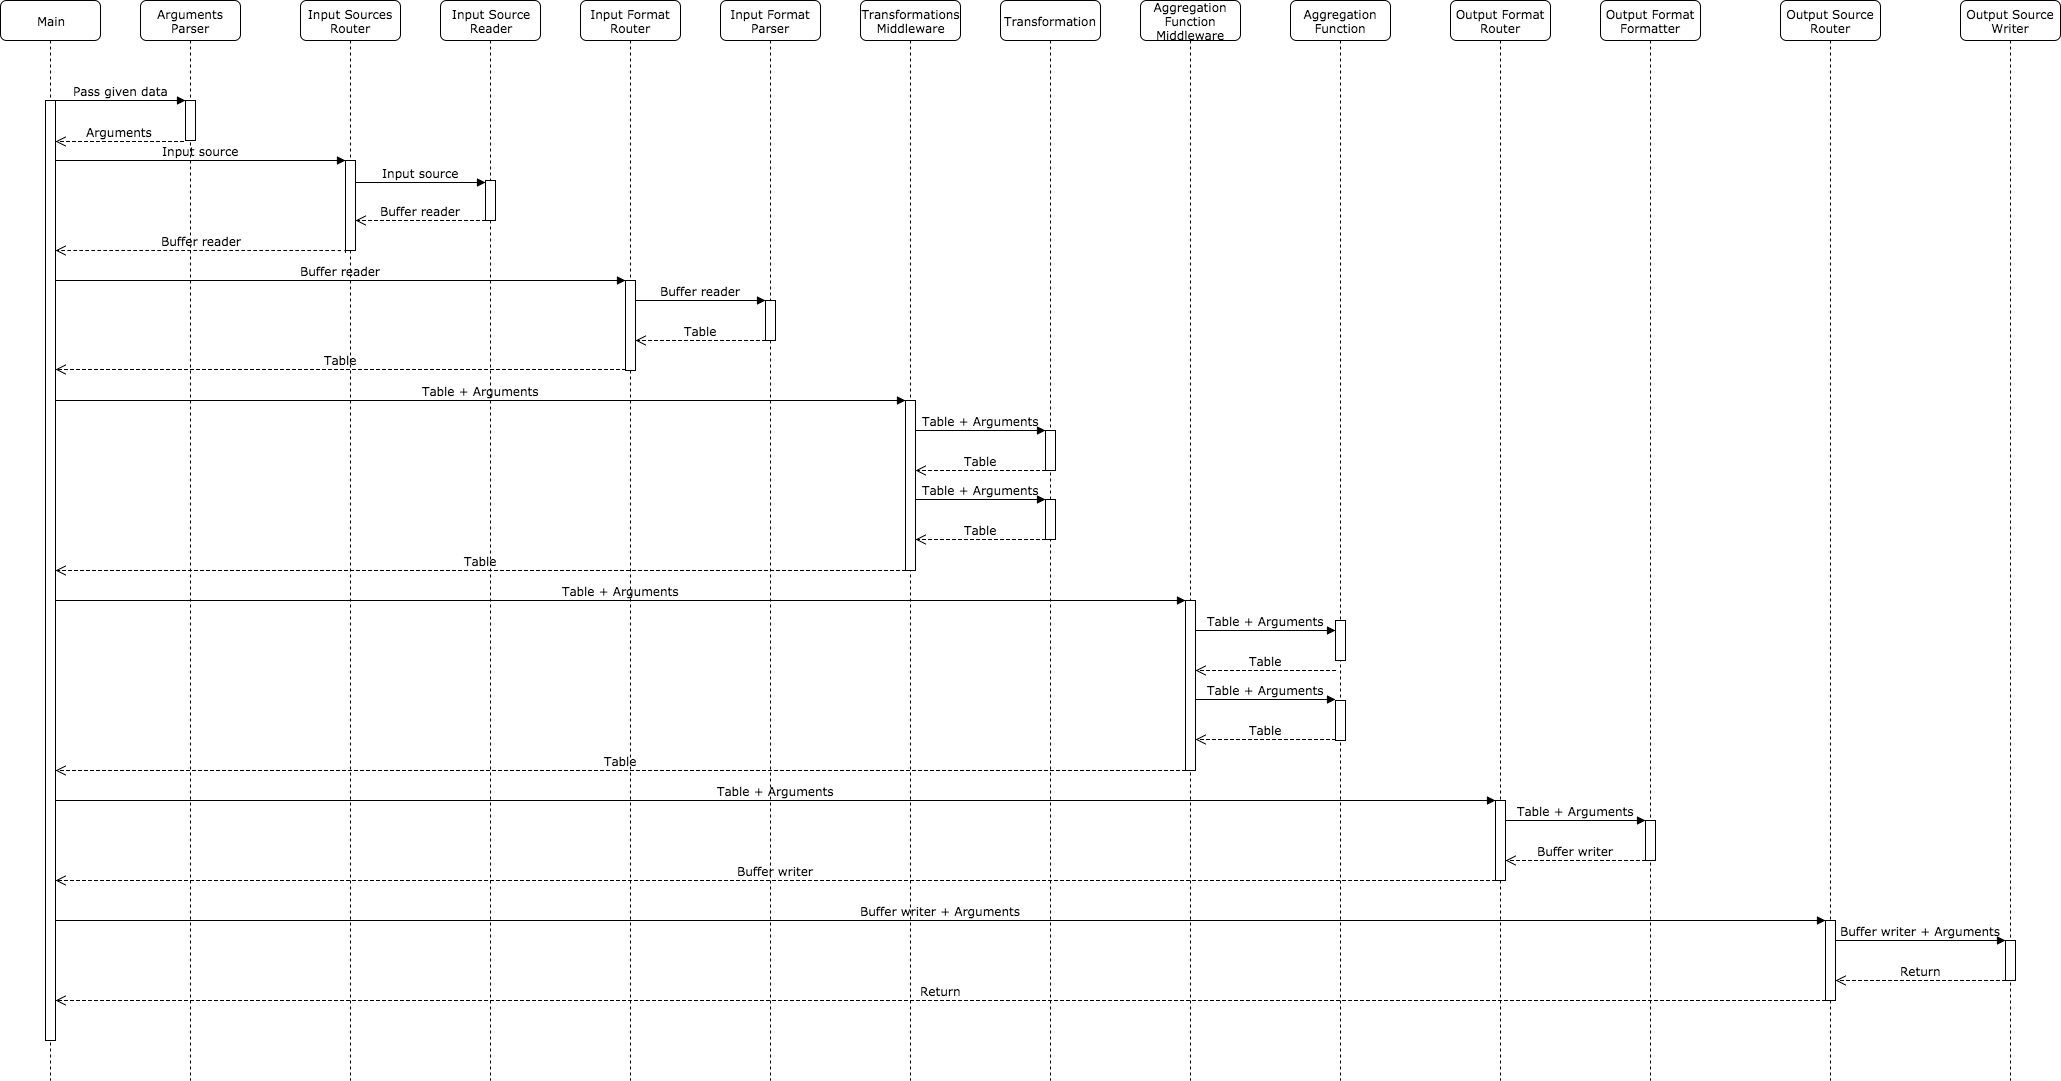
\includegraphics[width=\textheight, angle=90]{data_processing_flow_chart}
  \caption{Diagram toka obrade podataka}
  \label{data_processing_flow_chart}
\end{figure}

\chapter{Ostvareno rješenje}

\section{Korištene tehnologije}

Rješenje je implementirano u programskom jeziku Rust \cite{rust_lang_page}.

Rust je sistemski programski jezik (prevodi se direktno u procesorske
naredbe) funkcijske paradigme s naglaskom na sigurnost izvršavanja programa.
Program napisan u Rustu može isključivo imati implementacijske greške u pogledu
algoritamskih grešaka. Prevoditelj tijekom kompilacije programa (eng. compile
time) provjerava postoji li mogućnost stanja utrke (eng. race condition), te
pristupa li se podacima na način koji ne osigurava njihov integritet tijekom
izvođenja na vise dretva. Dodatno, jezik implementira koncept predivljivog
životnog vijeka varijabli stoga se programer ne mora ručno brinuti o alokaciji
i dealokaciji memorije, a ne uvodi se potreba za sakupljačem smeća (eng.
garbage collector) koji znatno utječu na performanse programa.

Važno je za napomenuti da Rust navedene garancije postiže uvođenjem nekolicine
novih koncepata. Najbitniji je koncept vlasništva (eng. ownership) pošto utječe
na sve varijable. Koncept vlasništva zabranjuje korištenje neke varijable kao
argument funkciji ako je ona prethodno bila korištena kao argument drugoj
funkciji. Potom slijedi koncept posuđivanja (eng. borrowing) koji dozvoljava
postojanje referenci na varijablu. Svaka varijabla može imati ili beskonačno
referenci za čitanje ili jednu referencu za čitanje i pisanje. Konačno, koncept
vremena života (eng. life time). Vrijeme života određuje u kojem će se trenutku
dealocirati rezultat funkcije. \ povezuje trenutak dealociranja ulaznih i
izlazne reference funkcije. Rust također posuđuje koncepte iz ostalih
funkcijskih programskih jezika poput ne posjedovanja Null vrijednosti, Maybe
vrijednosti iz Haskella \cite{haskell_lang_page}, prepoznavanje uzoraka
(eng. pattern matching) iz Erlanga \cite{erlang_lang_page} i mnoge druge.

Rust je razvijen od Mozilla organizacije kao alat za izradu Internetskog
preglednika koji ne će imati sigurnosne propuste. Početni fokus je bio
napraviti virtualni stroj za JavaScript međutim nakon 2015 se fokus proširio na
implementaciju HTML parsera, URL parsera, H264 i MP3 dekodera stoga u ekosustavu
postoji veliki broj programskih knjižnica otvorenog koda koje su inkorporirane
u konačno rješenje.

Za prevođenje izvornog koda se koristi rustc prevoditelj koji je baziran na
LLVM projektu \cite{llvm_page}. Uz sam prevoditelj se koristi alat zvan
Cargo \cite{cargo_documentation}
koji je kombinacija managera programskih knjižnica o kojima program ovisi i
sustava za optimizaciju kompilacije sličnom sustavu
Make \cite{make_documentation}.

\section{Korištene programske knjižnice}

\subsection{html5ever}

html5ever \cite{html5ever_repository} je HTML parser razvijen od Mozille za
njihov novi browser zvan Servo.
Cilj knjižnice je napraviti HTML parser bez sigurnosnih propusta kakvi su
prisutni u C implementacijama.

Može parsirati i serijalizirati HTML prema HTML5 specifikaciji, tokenizirati ga,
the pretvoriti u objektno stablo. Najbitnija usluga koju nudi je sanitizacija
HTML-a, naime moderni Internet pretrživati sanitiziraju HTML s web stranica
koje posjećuju. Stranice često sadrže sintaktičke greške u HTML kodu te kako
bi ih pretraživač mogao prikazati mora prvo popraviti sintaksu HTML-a,
odnosno mora ga sanitizirati. Osim sanitizacije, bitno svojstvo ove
knjižnice je da obraduje podatke kao tok podataka (eng. stream) sto znatno
smanjuje potrošnju memorije.

Ova knjižnice se koristi u konačnom rješenju za parsiranje HTML koda u
internu reprezentaciju tablica.

\subsection{ncurses}

ncurses \cite{ncurses_documentation} je programska knjižnice koja omogućava
programeru kreaciju
tekstualnih grafičkih sučelja neovisnih o terminalu na kojem se izvode te
visoko optimiziranim za korištenje u programskim sučeljima koja se koriste na
daljinu (npr. pomoću programa ssh).

ncurses je zapravo treća iteracija ove knjižnice. Prva iteracija se zvala
curses i bila je razvijena na sveučilištu u Californiji - Berkley s namjenom
da se koristi za tekstualne igre u operativnom sustavu BSD. curses je stekao
nepredviđenu popularnost sto je ponukalo Bell Labs da 1980. razvije svoju
verziju knjižnice i integrira ju u operativni sustav System V. Druga
iteracija je bila pcurses, razvijena 1986. od Pavel Curtisa kao besplatna
verzija curses knjižnice. ncurses je unaprijeđena verzija pcursesa objavljena
1993. koja dodaje podršku za izbornike i padajuće izbornike, te je kompatibilna
s originalnom verzijom curses knjižnice.

Pomoću ove knjižnice je ostvareno grafičko sučelje rješenja. Omogućava lako
stvaranje prozora, crtanje tablica i izradu interaktivnih izbornika. Podržano
je na svim operativnim sustavim koji zadovoljavaju POSIX standard, te na
Windowsima (potrebno je instalirati dodatne programske pakete).

Grafičko sučelje koje je implementirano pomoću ove knjižnice je portabilno u
smislu da se ponaša jednako na svim operativnim sustavima, kernelima i
terminalima. Na modernim terminalima je moguće koristiti miš za selekciju
izbornika ili dugmadi stoga se rješenje ponaša kao aplikacija s grafičkim
sučeljem iako je ono zapravo implementirano kao tekst.

U konačnom rješenju se koristi ncurses-rs \cite{ncurses_rs_repository} verzija
knjižnice koja omotava C knjižnicu u Rust kod.

\subsection{hyper}

Hyper \cite{hyper_repository} je programska knjižnica za komunikaciju HTTP
protokolom.

Hyper se smatra modernom i elegantnom apstrakcijom iznad HTTP protokola.
Nudi direktno sučelje iznad protokola za implementaciju klijenata i
poslužitelja.
Ne ovisi o vanjskim knjižnicama ta je po performancama brze od libcurla
(knjižnica koja dolazi standardno u velikom broju operativnih sustava).

U konačnom rješenju Hyper se koristi za dohvat podataka s web stranica.

\section{Uputstva za instalaciju rješenja}

Konačno rješenje je moguće preuzeti s poveznice
\url{https://github.com/stankec/give_me_tables/releases/latest}

Potrebno je preuzeti verziju binarne datoteke koja odgovara arhitekturi i
kernelu računala na kojem će se program izvoditi. Po preuzimanju potrebno je
binarnoj datoteci dati pravo izvođenja i preseliti ju u direktorij u kojem
operativni sustav traži aplikacije.

Konkretan postupak instalacije najnovije inačice rješenja za računalo sa
64-bitnim procesorom na x86 arhitekturi i operativnim sustavom s Linux kernelom:

\begin{lstlisting}
curl https://github.com/stankec/give_me_tables\
/releases/download/latest/\
give_me_tables-x86_64-linux-gnu > ~/give_me_tables
chmod +x ~/give_me_tables
sudo mv ~/give_me_tables /usr/bin/give_me_tables
\end{lstlisting}

Alternativno ako korisnik želi pregledati kod aplikacije i uvjeriti se da nije
izmjenjen, moguće je i prevesti aplikaciju na računalu koje će ju izvoditi:

\begin{lstlisting}
git clone git@github.com:stankec/give_me_tables.git
cd give_me_tables
curl https://sh.rustup.rs -sSf | sh
rustup update
rustup install nightly
rustup default nightly
cargo build --release
mv target/release/give_me_tables /usr/bin/give_me_tables
\end{lstlisting}

\section{Uputstva za korištenje rješenja}

Po instalaciji rješenja će korisnik u svojem programskom sučelju
(npr. terminalu) imati dostupnu naredbu "give\_me\_tables". Pokretanje naredbe
direktno bez argumenata će ispisati upozorenje sa šturim uputstvima za
korištenje. Od tuda je moguće vidjeti koje tipove argumenata je moguće
proslijediti, te koji argumenti su očekivani. Na kraju će nas uputiti da za
detaljna uputstva proslijedimo zastavicu "--help" ili "-h".

Po ponovno pokretanju rješenja sa zastavicom "--help" prikazat će se detaljna
uputstva koja izlistavaju ime aplikacije, verziju aplikacije, osobu koja ju
održava, kratki opis, uzorak unosa podataka, moguće zastavici, njihove kratice
i čemu služe, te moguće opcije, njihove kratice, čemu služe i kako ih se
koristi.

Bitno je za napomenuti da aplikacija iznosi opcije "input-file" i "url", te
argument "INPUT" kao obavezne iako je potrebno definirati samo jednu od
navedenih opcija.

Postoji nekolicina informativnih zastavica poput "license" koji ispisuje
licencu po kojom se konačno rješenje može koristiti i distribuirati, potom
"list-aggregation-functions" koji
ispisuje sve dostupne agregacijske funkcije i njihove opise, analogno
agregacijskim funkcijama postoji "list-transformations" koji ispisuje sve
dostupne transformacije s njihovom opisom. Konačno postoji "list-tables"
koji će samo ispisati kratki pregled svih postojećih tablica iz ulaznog
dokumenta. Ako postoji potreba za detaljnim uvidom u ponašanje rješenja moguće
je proslijediti "verbose" zastavicu do tri puta sto će imati za posljedicu da
će se ispisivati greške, upozorenja i generalne informacije tijekom izvođenja.

Postoji i nekolicina opcija koje utječu na ponašanje samog programa. Npr.
"input-file" pomoću koje se specificira iz koje datoteke se čitaju ulazni
podaci, potom "url" koji specificira s kojeg URL-a se čitaju ulazni podati, te
"output-file" koji specificira u koju datoteku se zapisuje rezultat (ako se ova
opcija ne navede se rezultat ispise na standardni izlaz).

Opcije namijenjene manipulaciji ulaznih podataka su "aggregation-function" i
"transformation". One očekuju do 3 argumenta odvojena zarezom (ime funkcije ili
transformacije, ime stupca i broj retka) koji specificiraju nad kojim podacima
se funkcija izvodi.

Primjer naredbe za ispisivanje svih postojećih tablica s web stranice
fer.unizg.hr uz ispisivanje informacija o radu:

\begin{lstlisting}
give_me_tables -vvv --url https://fer.unizg.hr --list-tables
\end{lstlisting}

Ako želimo predati podatke kroz standardni ulaz, transponirati tablicu i
izračunati maksimalnu vrijednost drugog reda i pohraniti rezultat u datoteku
možemo izvesti sljedeću naredbu

\begin{lstlisting}
curl -L https://fer.unizg.hr | give_me_tables \
--transformation "transpose" --aggregation-function "max,A,2" \
--output-file output.csv
\end{lstlisting}

Ako želimo pročitati podatke iz datoteke možemo izvesti sljedeću naredbu:

\begin{lstlisting}
curl -L https://fer.unizg.hr > fer_web.html && \
give_me_tables -vvv --list-tables --input-file ./fer_web.html
\end{lstlisting}



\chapter{Zaključak}

Konačno rješenje je zadovoljilo osnovne potrebe zadatka, međutim moguće ga je
dodatno unaprijediti u budućnosti.

Prvo i očito unaprjeđenje je implementacija dodatnih agregacijskih funkcija
poput count, median, mode, sign i drugih, te transformacija poput move i
reverse.

Potom, prethodno je navedeno potencijalno proširenje na prihvaćanje PDF
datoteka kao ulaznih datoteka. Analogno tome, implementacija dodatnih
izlaznih formata datoteka poput xls, xslx i ods.

Sa strane distribucije rješenja. Za povećanje povjerenja između korisnika i
distributera bi se prevođenje binarne datoteke trebale potpisati s GPG
privatnim ključem. A za olakšanje instalacije bi se trebao podignuti
distribucijski poslužitelj za apt \cite{apt_wiki}, yum \cite{yum_wiki} i
pacman \cite{pacman_wiki} programske managere.

Rješenje, kao i njegov izvorni kod, je javno objavljeno na sljedećoj
poveznici \url{https://github.com/stankec/give_me_tables} pod verzijom 3 GNU
javne license \cite{gplv3_license}.

GNU javna licenca verzija 3 (skraćeno GPLv3) obvezuje korisnike da ukoliko
žele komercijalno koristiti rješenje moraju sve promjene koje su napravili na
izvornom kodu javno objaviti, te štiti načela pokreta za besplatne programe
\cite{free_software_movement_manifesto} (eng. Free Software Movement).


\bibliography{zavrsni}
\bibliographystyle{fer}

\begin{sazetak}

Proučiti i opisati dostupne sustave za izdvajanje tabličnih podataka iz
polu-strukturiranih dokumenata kao što su web-stranice ili PDF dokumenti.
Osmisliti i ostvariti sustav za izdvajanje strukturiranih tabličnih podataka iz
navedenih dokumenata s naglaskom na web-stranice.
Sustav treba izložiti svoje funkcionalnosti koristeći sučelje naredbenog retka
za koje je potrebno osmisliti skup naredbi za jednostavni interaktivni rad.
Nadalje, ostvariti i osnovno programsko sučelje sustava. Prikupiti skup
web-stranica za ispitivanje rada sustava te ocijeniti uspješnost izdvajanja
tabličnih podataka s obzirom na složenost strukture ulaznog dokumenta. Opisati
izgrađeni sustav, navesti upute za postavljanje, načine korištenja, navesti
literaturu i primljenu pomoć.

\kljucnerijeci{}
\end{sazetak}

\engtitle{System for Tabular Data Extration from Web-pages}
\begin{abstract}

Study and describe available systems for extraction of tabular data from
semi-structured documents like web sites or PDF documents. Think of and
implement a system for extracting of structured tabular data from the types of
documents mentioned above with an emphesys on web sites.
The system should be implemented as a command line interface with a set of
commands for interactive use. Aggregate a set of web sites for testing the
effectivnes of data extraction regarding the com[plexety of the input.
Describe the created system, write setup instrunctions, usage instructions,
cite the literature used and any help received.

\keywords{}
\end{abstract}

\end{document}
